\documentclass[ignorenonframetext,]{beamer}
\usetheme{Madrid}
\usecolortheme{whale}
\setbeamertemplate{caption}[numbered]
\setbeamertemplate{caption label separator}{:}
\setbeamercolor{caption name}{fg=normal text.fg}
\usepackage{amssymb,amsmath}
\usepackage{ifxetex,ifluatex}
\usepackage{fixltx2e} % provides \textsubscript
\usepackage{lmodern}
\ifxetex
  \usepackage{fontspec,xltxtra,xunicode}
  \defaultfontfeatures{Mapping=tex-text,Scale=MatchLowercase}
  \newcommand{\euro}{€}
\else
  \ifluatex
    \usepackage{fontspec}
    \defaultfontfeatures{Mapping=tex-text,Scale=MatchLowercase}
    \newcommand{\euro}{€}
  \else
    \usepackage[T1]{fontenc}
    \usepackage[utf8]{inputenc}
      \fi
\fi
% use upquote if available, for straight quotes in verbatim environments
\IfFileExists{upquote.sty}{\usepackage{upquote}}{}
% use microtype if available
\IfFileExists{microtype.sty}{\usepackage{microtype}}{}
\usepackage{longtable,booktabs}
\usepackage{caption}
% These lines are needed to make table captions work with longtable:
\makeatletter
\def\fnum@table{\tablename~\thetable}
\makeatother
\usepackage{graphicx}
\makeatletter
\def\maxwidth{\ifdim\Gin@nat@width>\linewidth\linewidth\else\Gin@nat@width\fi}
\def\maxheight{\ifdim\Gin@nat@height>\textheight0.8\textheight\else\Gin@nat@height\fi}
\makeatother
% Scale images if necessary, so that they will not overflow the page
% margins by default, and it is still possible to overwrite the defaults
% using explicit options in \includegraphics[width, height, ...]{}
\setkeys{Gin}{width=\maxwidth,height=\maxheight,keepaspectratio}

% Comment these out if you don't want a slide with just the
% part/section/subsection/subsubsection title:
\AtBeginPart{
  \let\insertpartnumber\relax
  \let\partname\relax
  \frame{\partpage}
}
\AtBeginSection{
  \let\insertsectionnumber\relax
  \let\sectionname\relax
  \frame{\sectionpage}
}
\AtBeginSubsection{
  \let\insertsubsectionnumber\relax
  \let\subsectionname\relax
  \frame{\subsectionpage}
}

\setlength{\parindent}{0pt}
\setlength{\parskip}{6pt plus 2pt minus 1pt}
\setlength{\emergencystretch}{3em}  % prevent overfull lines
\setcounter{secnumdepth}{0}
\usepackage[russian]{babel}
\author[Эконометрика. Лекция 1]{Эконометрика. Лекция 1}

\title{Метод наименьших квадратов}
\date{}

\begin{document}
\frame{\titlepage}

\begin{frame}{Эконометрика на одном слайде :)}

\begin{block}{Вопросы:}

\begin{itemize}
\itemsep1pt\parskip0pt\parsep0pt
\item
  Как устроен мир? Как переменная \(x\) влияет на переменную \(y\)?
\item
  Что будет завтра? Как спрогнозировать переменную \(y\)?
\end{itemize}

\end{block}

\begin{block}{Ответ:}

Модель --- формула для объясняемой переменной

\end{block}

\begin{block}{Например:}

\begin{itemize}
\itemsep1pt\parskip0pt\parsep0pt
\item
  \(y_i=\beta_1+\beta_2 x_i + \varepsilon_i\) 
\end{itemize}

\end{block}

\end{frame}

\begin{frame}{Основные типы данных:}

\begin{itemize}
\itemsep1pt\parskip0pt\parsep0pt
\item
  Временные ряды
\item
  Перекрёстные данные
\item
  Панельные данные
\end{itemize}

Есть много-много других!

\end{frame}

\begin{frame}{Временные ряды}

Данные по России:

\begin{longtable}[c]{@{}lll@{}}
\toprule
Год & Население & Безработица\tabularnewline
\midrule
\endhead
2010 & 142962 & 7.4\tabularnewline
2011 & 142914 & 6.5\tabularnewline
2012 & 143103 & 5.5\tabularnewline
2013 & 143395 & 5.5\tabularnewline
\bottomrule
\end{longtable}

\end{frame}

\begin{frame}{Перекрёстная выборка}

Результаты зимних Олимпийских игр 2014:

\begin{longtable}[c]{@{}llll@{}}
\toprule
Страна & Золото & Серебро & Бронза\tabularnewline
\midrule
\endhead
Россия & 13 & 11 & 9\tabularnewline
Норвегия & 11 & 5 & 10\tabularnewline
Канада & 10 & 10 & 5\tabularnewline
США & 9 & 7 & 12\tabularnewline
\bottomrule
\end{longtable}

\end{frame}

\begin{frame}{Панельные данные}

Cочетание первых двух: данные по нескольким переменным для множества
объектов в разные моменты времени

\end{frame}

\begin{frame}{Данные --- обозначения}

\begin{itemize}
\itemsep1pt\parskip0pt\parsep0pt
\item
  Одна зависимая, объясняемая, переменная: \(y\)
\item
  Несколько регрессоров, объясняющих, переменных: \(x\), \(z\),
  \(\ldots\)
\item
  По каждой переменной \(n\) наблюдений: \(y_1\), \(y_2\), \(\ldots\),
  \(y_n\)
\end{itemize}

\end{frame}

\begin{frame}{Данные --- пример}

Исторические данные 1920-х годов :)

\begin{longtable}[c]{@{}rr@{}}
\toprule
Длина тормозного пути (м), \(y_i\) & Скорость машины (км/ч),
\(x_i\)\tabularnewline
\midrule
\endhead
0.6 & 6.44\tabularnewline
3.0 & 6.44\tabularnewline
1.2 & 11.27\tabularnewline
\ldots{} & \ldots{}\tabularnewline
\bottomrule
\end{longtable}

\end{frame}

\begin{frame}{Всегда изображайте данные!}

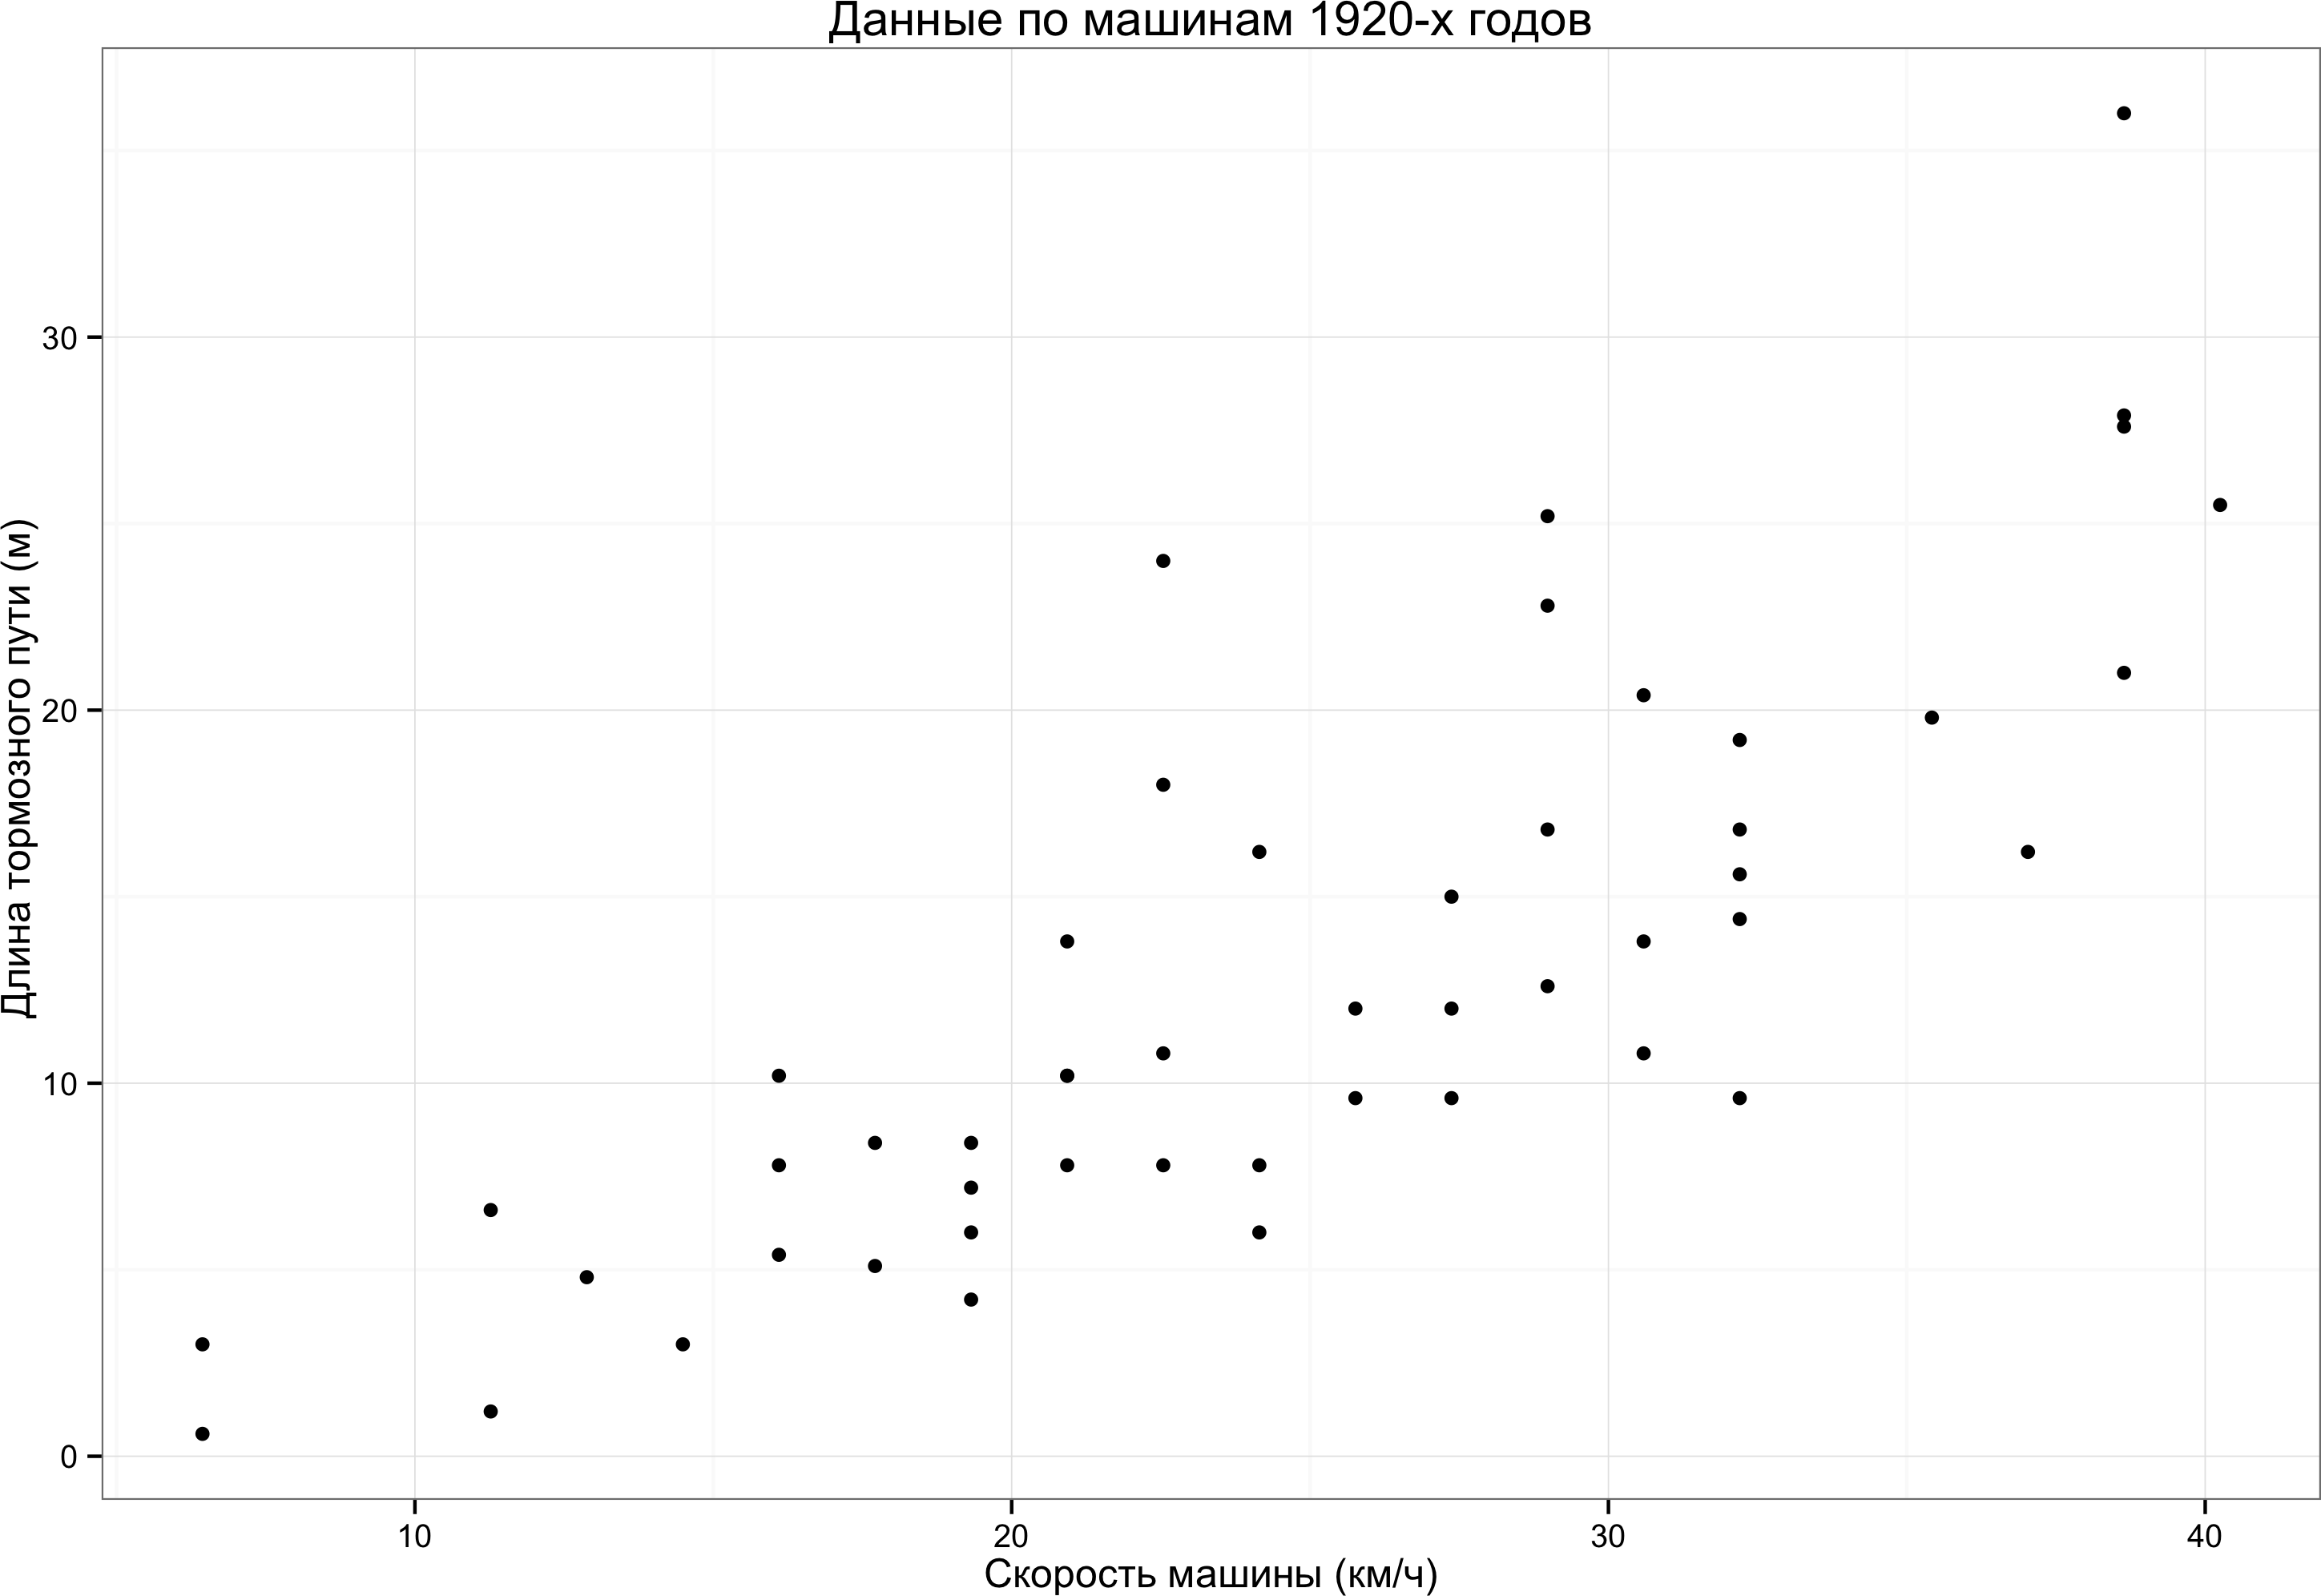
\includegraphics{lec_01_files/figure-beamer/unnamed-chunk-3-1.png}

\end{frame}

\begin{frame}{Модель:}

Пример: \(y_i=\beta_1 + \beta_2 x_i + \varepsilon_i\)

\begin{itemize}
\itemsep1pt\parskip0pt\parsep0pt
\item
  Наблюдаемые переменные: \(y\), \(x\)
\item
  Неизвестные параметры: \(\beta_2\), \(\beta_2\)
\item
  Случайная составляющая, ошибка: \(\varepsilon\)
\end{itemize}

\begin{block}{План действий}

\begin{itemize}
\itemsep1pt\parskip0pt\parsep0pt
\item
  придумать адекватную модель\\
\item
  получить оценки неизвестных параметров: \(\hat{\beta}_1\),
  \(\hat{\beta}_2\)\\
\item
  прогнозировать, заменив неизвестные параметры на оценки:\\\[
  \hat{y}_i=\hat{\beta}_1 + \hat{\beta}_2 x_i
  \]
\end{itemize}

\end{block}

\end{frame}

\begin{frame}{Метод наименьших квадратов}

\begin{itemize}
\itemsep1pt\parskip0pt\parsep0pt
\item
  Способ получить оценки неизвестных параметров модели исходя из
  реальных данных.
\end{itemize}

Ошибка прогноза: \(\hat{\varepsilon}_i=y_i-\hat{y}_i\).

Сумма квадратов ошибок прогноза: \[
Q(\hat{\beta}_1,\hat{\beta}_2)=\sum_{i=1}^n \hat{\varepsilon}_i^2=\sum_{i=1}^n (y_i-\hat{y}_i)^2
\]

Суть МНК: В качестве оценок взять такие \(\hat{\beta}_1\),
\(\hat{\beta}_2\), при которых сумма квадратов ошибок прогноза, \(Q\),
минимальна.

\end{frame}

\begin{frame}{Пример с машинами:}

Фактические данные:

\(x_1=6.68\), \(x_2=6.68\), \ldots{},

\(y_1=0.6\), \(y_2=3\), \ldots{}

Модель: \(y_i=\beta_1+\beta_2 x_i+\varepsilon_i\). Формула для
прогнозов: \(\hat{y}_i=\hat{\beta}_1 + \hat{\beta}_2 x_i\)

Сумма квадратов ошибок прогнозов: \(Q=\sum_{i=1}^n (y_i-\hat{y}_i)^2\)

\[
Q=(0.6-\hat{\beta}_1-\hat{\beta}_2 6.68)^2+(3-\hat{\beta}_1-\hat{\beta}_2 6.68)^2+...
\]

Точка минимума, найдена в R: \(\hat{\beta}_1=-5.3\),
\(\hat{\beta}_2=0.7\):

Формула для прогнозов: \(\hat{y}_i=-5.3 + 0.7 x_i\)

\end{frame}

\begin{frame}{Простой пример {[}у доски{]}}

\begin{longtable}[c]{@{}rrr@{}}
\toprule
Имя & Вес (кг), \(y_i\) & Рост (см), \(x_i\)\tabularnewline
\midrule
\endhead
Вася & 60 & 170\tabularnewline
Коля & 70 & 170\tabularnewline
Петя & 80 & 181\tabularnewline
\bottomrule
\end{longtable}

Оцените
модели:\\\(y_i=\beta x_i +\varepsilon_i\),\\\(y_i=\beta_1+\beta_2 x_i +\varepsilon_i\)

Маленькая подготовка: \(n\bar{x}=\sum_i x_i=\sum_i \bar{x}\),
\(\sum_i (x_i - \bar{x})=0\).

\end{frame}

\begin{frame}{Готовые формулы МНК. Регрессия на константу}

В модели \(y_i=\beta +\varepsilon_i\)

\[
\hat{\beta}=\bar{y}
\]

Интерпретация:

В модели без объясняющих переменных наилучший прогноз --- это среднее
значение зависимой переменной

\end{frame}

\begin{frame}{Готовые формулы МНК. Парная регрессия}

В модели \(y_i=\beta_1+\beta_2 x_i +\varepsilon_i\)

\[
\hat{\beta}_2=\frac{\sum (x_i-\bar{x})(y_i-\bar{y})}{\sum (x_i-\bar{x})^2}
\] \[
\hat{\beta}_1=\bar{y}-\hat{\beta}_2\bar{x}
\]

Интерпретация:

Точка \((\bar{x},\bar{y})\) лежит на линии регрессии
\(\hat{y}=\hat{\beta}_1+\hat{\beta}_2 x\)

\end{frame}

\begin{frame}{Терминология и обозначения:}

\(y_i\) --- зависимая, объясняемая, переменная

\(x_i\) --- регрессор, объясняющая переменная

\(\varepsilon_i\) --- ошибка, ошибка модели, случайная составляющая

\(\hat{y}_i\) --- прогноз, прогнозное значение

\(\hat{\varepsilon}_i=y_i-\hat{y}_i\) --- остаток, ошибка прогноза

\(RSS=\sum_{i=1}^n \hat{\varepsilon}_i^2\) --- сумма квадратов остатков

\end{frame}

\begin{frame}{Графическая иллюстрация (чудо-доска)}

!показать, что регрессия проходит через среднюю точку

\end{frame}

\begin{frame}{Много объясняющих переменных {[}у доски{]}}

\(y_i=\beta_1+\beta_2 x_i +\beta_3 z_i+\varepsilon_i\)

Выпишем систему уравнений для оценок \(\hat{\beta}_1\),
\(\hat{\beta}_2\), \(\hat{\beta}_3\)

\[
\begin{cases}
\sum \hat{\varepsilon}_i \cdot 1 =0 \\
\sum \hat{\varepsilon}_i \cdot x_i =0 \\
\sum \hat{\varepsilon}_i \cdot z_i =0
\end{cases}
\]

\end{frame}

\begin{frame}{Суммы квадратов}

\begin{itemize}
\item
  Сумма квадратов остатков \[
  RSS=\sum \hat{\varepsilon}_i^2
  \]
\item
  Общая сумма квадратов \[
  TSS=\sum (y_i-\bar{y})^2
  \]
\item
  Объясненная сумма квадратов \[
  ESS=\sum (\hat{y}_i-\bar{y})^2
  \]
\end{itemize}

\end{frame}

\begin{frame}{Абсолютный ликбез по линейной алгебре}

Вектора: \(y\), \(x\), \(\hat{y}\), \(\varepsilon\), \ldots

\[
y=\begin{pmatrix}
y_1 \\
y_2 \\
\vdots \\
y_n
\end{pmatrix}\;
x=\begin{pmatrix}
x_1 \\
x_2 \\
\vdots \\
x_n
\end{pmatrix}\;
\hat{\varepsilon}=\begin{pmatrix}
\hat{\varepsilon}_1 \\
\hat{\varepsilon}_2 \\
\vdots \\
\hat{\varepsilon}_n
\end{pmatrix}\;
\vec{1}=\begin{pmatrix}
1 \\
1 \\
\vdots \\
1
\end{pmatrix}
\]

В нашей модели:
\(\hat{y}=\hat{\beta}_1 \cdot \vec{1}+\hat{\beta}_2 \cdot x +\hat{\beta}_3 \cdot z\)

\end{frame}

\begin{frame}{Матрица всех регрессоров}

\[
X=\begin{pmatrix}
1 & x_1 & z_1 \\
1 & x_2 & z_2 \\
\vdots \\
1 & x_n & z_n 
\end{pmatrix}
\]

\end{frame}

\begin{frame}{Длина вектора}

Длина вектора, \(|y|=\sqrt{y_1^2+y_2^2+\ldots+ y_n^2}\)

Квадрат длины вектора, \(|y|^2=y_1^2+y_2^2+\ldots + y_n^2=\sum_i y_i^2\)

Примеры:\\\(RSS=\sum \hat{\varepsilon}_i^2\) --- квадрат длины вектора
\(\hat{\varepsilon}\)\\\(TSS=\sum (y_i-\bar{y})^2\) --- квадрат длины
вектора \((y-\bar{y}\cdot \vec{1})\)

\(\begin{pmatrix} y_1-\bar{y} \\ y_2-\bar{y} \\ \vdots \\ y_n-\bar{y} \end{pmatrix} = \begin{pmatrix} y_1 \\ y_2 \\ \vdots \\ y_n \end{pmatrix} - \bar{y}\begin{pmatrix} 1 \\ 1 \\ \vdots \\ 1 \end{pmatrix}=y-\bar{y}\cdot \vec{1}\)

\end{frame}

\begin{frame}{Скалярное произведение двух векторов:}

\[
(x,y)=|x|\cdot |y|\cdot cos(x,y)
\]

\[
(x,y)=x_1 y_1 +x_2 y_2 +\ldots+ x_n y_n=\sum_i x_i y_i
\]

Условие перпендикулярности:

\[
x \perp y  \Leftrightarrow  \sum_i x_i y_i=0
\]

т.к. \(cos(90^\circ)=0\).

\end{frame}

\begin{frame}{Иллюстрация для регрессии на константу {[}у доски{]}}

Модель: \(y_i=\beta + \varepsilon_i\)

\end{frame}

\begin{frame}{Геометрическая интерпретация условий первого порядка}

\[
\begin{cases}
\sum \hat{\varepsilon}_i \cdot 1 =0 \\
\sum \hat{\varepsilon}_i \cdot x_i =0 \\
\sum \hat{\varepsilon}_i \cdot z_i =0
\end{cases}\; \Leftrightarrow \;
\begin{cases}
\hat{\varepsilon}\perp \vec{1} \\
\hat{\varepsilon}\perp x \\
\hat{\varepsilon}\perp z \\
\end{cases}
\]

\end{frame}

\begin{frame}{Иллюстрация для множественной регрессии}

\end{frame}

\begin{frame}{Если в регрессию включён свободный член \(\beta_1\)}

Если в регрессию включён свободный член, \(y_i=\beta_1 + \ldots\), и
оценки МНК единственны, то:

\begin{itemize}
\itemsep1pt\parskip0pt\parsep0pt
\item
  \(\sum \hat{\varepsilon}_i=0\)\\
\item
  \(\sum y_i = \sum \hat{y}_i\)\\
\item
  \(\bar{y}=\bar{\hat{y}}\)\\
\item
  \(TSS=RSS+ESS\)
\end{itemize}

\end{frame}

\begin{frame}{Коэффициент детерминации --- простой показатель качества}

В моделях со свободным членом \(R^2=ESS/TSS\)

\(TSS\) --- общий разброс \(y\)\\\(ESS\) --- объясненный регрессорами
разброс\\\(R^2\) --- доля объясненного разброса в общем разбросе

Теорема. Если в регрессию включён свободный член,
\(y_i=\beta_1 + \ldots\), и оценки МНК единственны, то \(R^2\) равен
выборочной корреляции между \(y\) и \(\hat{y}\), т.е.

\[
R^2=(sCorr(y,\hat{y}))^2=\left(\frac{\sum (y_i-\bar{y})(\hat{y}_i-\bar{y})}{\sqrt{\sum(y_i-\bar{y})^2}\sqrt{\sum(\hat{y}_i-\bar{y})^2}}\right)^2
\]

\end{frame}

\begin{frame}{Явная формула для оценок коэффициентов}

Модель: \(y_i=\beta_1 + \beta_2 x_i +\beta_3 z_i +\varepsilon_i\)

\[
y=\begin{pmatrix}
y_1 \\
y_2 \\
\vdots \\
y_n 
\end{pmatrix}
\; X=\begin{pmatrix}
1 & x_1 & z_1 \\
1 & x_2 & z_2 \\
\vdots \\
1 & x_n & z_n 
\end{pmatrix}
\]

Линейная алгебра позволяет получить явные формулы:

\[
\hat{\beta}=(X'X)^{-1}X'y
\]

\end{frame}

\begin{frame}{Мораль}

УРА!!! МНК позволяет оценивать модели!!!

Предположив \(y_i=\beta_1 + \beta_2 x_i +\beta_3 z_i +\varepsilon_i\)

Получаем \(\hat{\beta}_1\), \(\hat{\beta}_2\), \(\hat{\beta}_3\)

\end{frame}

\begin{frame}{Вопросы}

\begin{itemize}
\item
  Как выбрать форму модели?
\item
  А будет ли решение задачи минимизации единственным?
\item
  А будет ли решение задачи минимизации вообще существовать?
\item
  А почему сумма квадратов остатков, а не, скажем, модулей?
\item
  А насколько точны полученные оценки?
\item
  \ldots{}
\end{itemize}

\end{frame}

\end{document}
